\documentclass[../main.tex]{subfiles}
\graphicspath{{\subfix{../images/}}}
\begin{document}

\subsubsection{Biological and Physiological Basis of Learning}

We are going to look at a few real and imaginary accelerators and inhibitors to learning, training and broadening our skills in more or less acute stress situations. They are going to be further elaborated on in the following sections:

\begin{itemize}
\item The biological and physiological basis of learning
\item Learning and it's effects
\item The definition of problem
\item Training and practicing
\item Tap into other areas of your brain
\item The meta--cognitive exercises, their mechanics and how they act on the brain.
  \item In the context above, explore possibilities to regulate stress with different psycho--motor capacities.
\end{itemize}

\section{In a Healthy Body Lives a Healthy Mind and Reciprocally}

The interaction between body and mind has been known for a long time.\index{body--mind interaction}
\emph{Mens sana in corpore sano} -- in a healthy body is a healthy mind -- was already known in antiquity.
Modern medicine confirmed this view of a human as whole being.
Humans can be seen as self--reinforcing feedback loop, as a system where body and mind influence each other.
Not only is it true that a healthy body allows an undisturbed, healthy thinking process, but the reverse is true as well.
My thought processes I can keep my body in motion, help it or weaken it, depending on the type of thought process happening.

Science knows a good amount about the processes in our brain, but there's no complete picture in sight yet. The statement by Jostein Gaarder still holds true: ``If the brain were simple enough for us to understand, then we would be too stupid to understand it.''

\epigraph{An untrained mind is more detrimental for health than an untrained body}{\textit{George Bernard Shaw}}
% I translated that

Body and mind react as a response to the other.
For instance it is incredibly hard to focus after a meal, while being exhausted or while having fever.
It is well known that certain times of the day are more conducive to the motivation and success of learning than others.
Further on, our positive or negative feelings have a big influence if we can recall the material later on.
We are astonished to hear that some cancer patients beat their disease, because they really want to achieve this. Scientists and researched know the phenomena that they are immune against disease and worries while they work on a fascinating project.

What is the link between the body--mind interaction and the topic of stress regulation? It helps to know for learners, that the process of thinking and learning has a physical--material and a mental--immaterial aspect to it.

In the brain, both system meet in the so called limbic system\index{limbic system}.
The name comes from it's position in the brain at the limbus, the border between the fore brain and the evolutionary older and less structured and deeper parts of the brain.
The limbic system is a sensitive interface between vegetative--bodily and mental--affective processes. It represents something like an emotional tribunal, which decides which information and stimuli are important and valuable for us.
If out of whatever reason it finds information to be important, it will hormonal color them pleasurable, so that they find easier access to our mind.\index{information!important}
On the other hand, if it finds them to be unimportant it then it puts up resistance by getting us annoyed. Such information has a harder time to find access into our memory.

How is information getting into our memory? Modern biology answers that question with a model of step wise committing to memory (encrypt, encode):\index{memory}

\begin{figure}[htb]
  \centering
  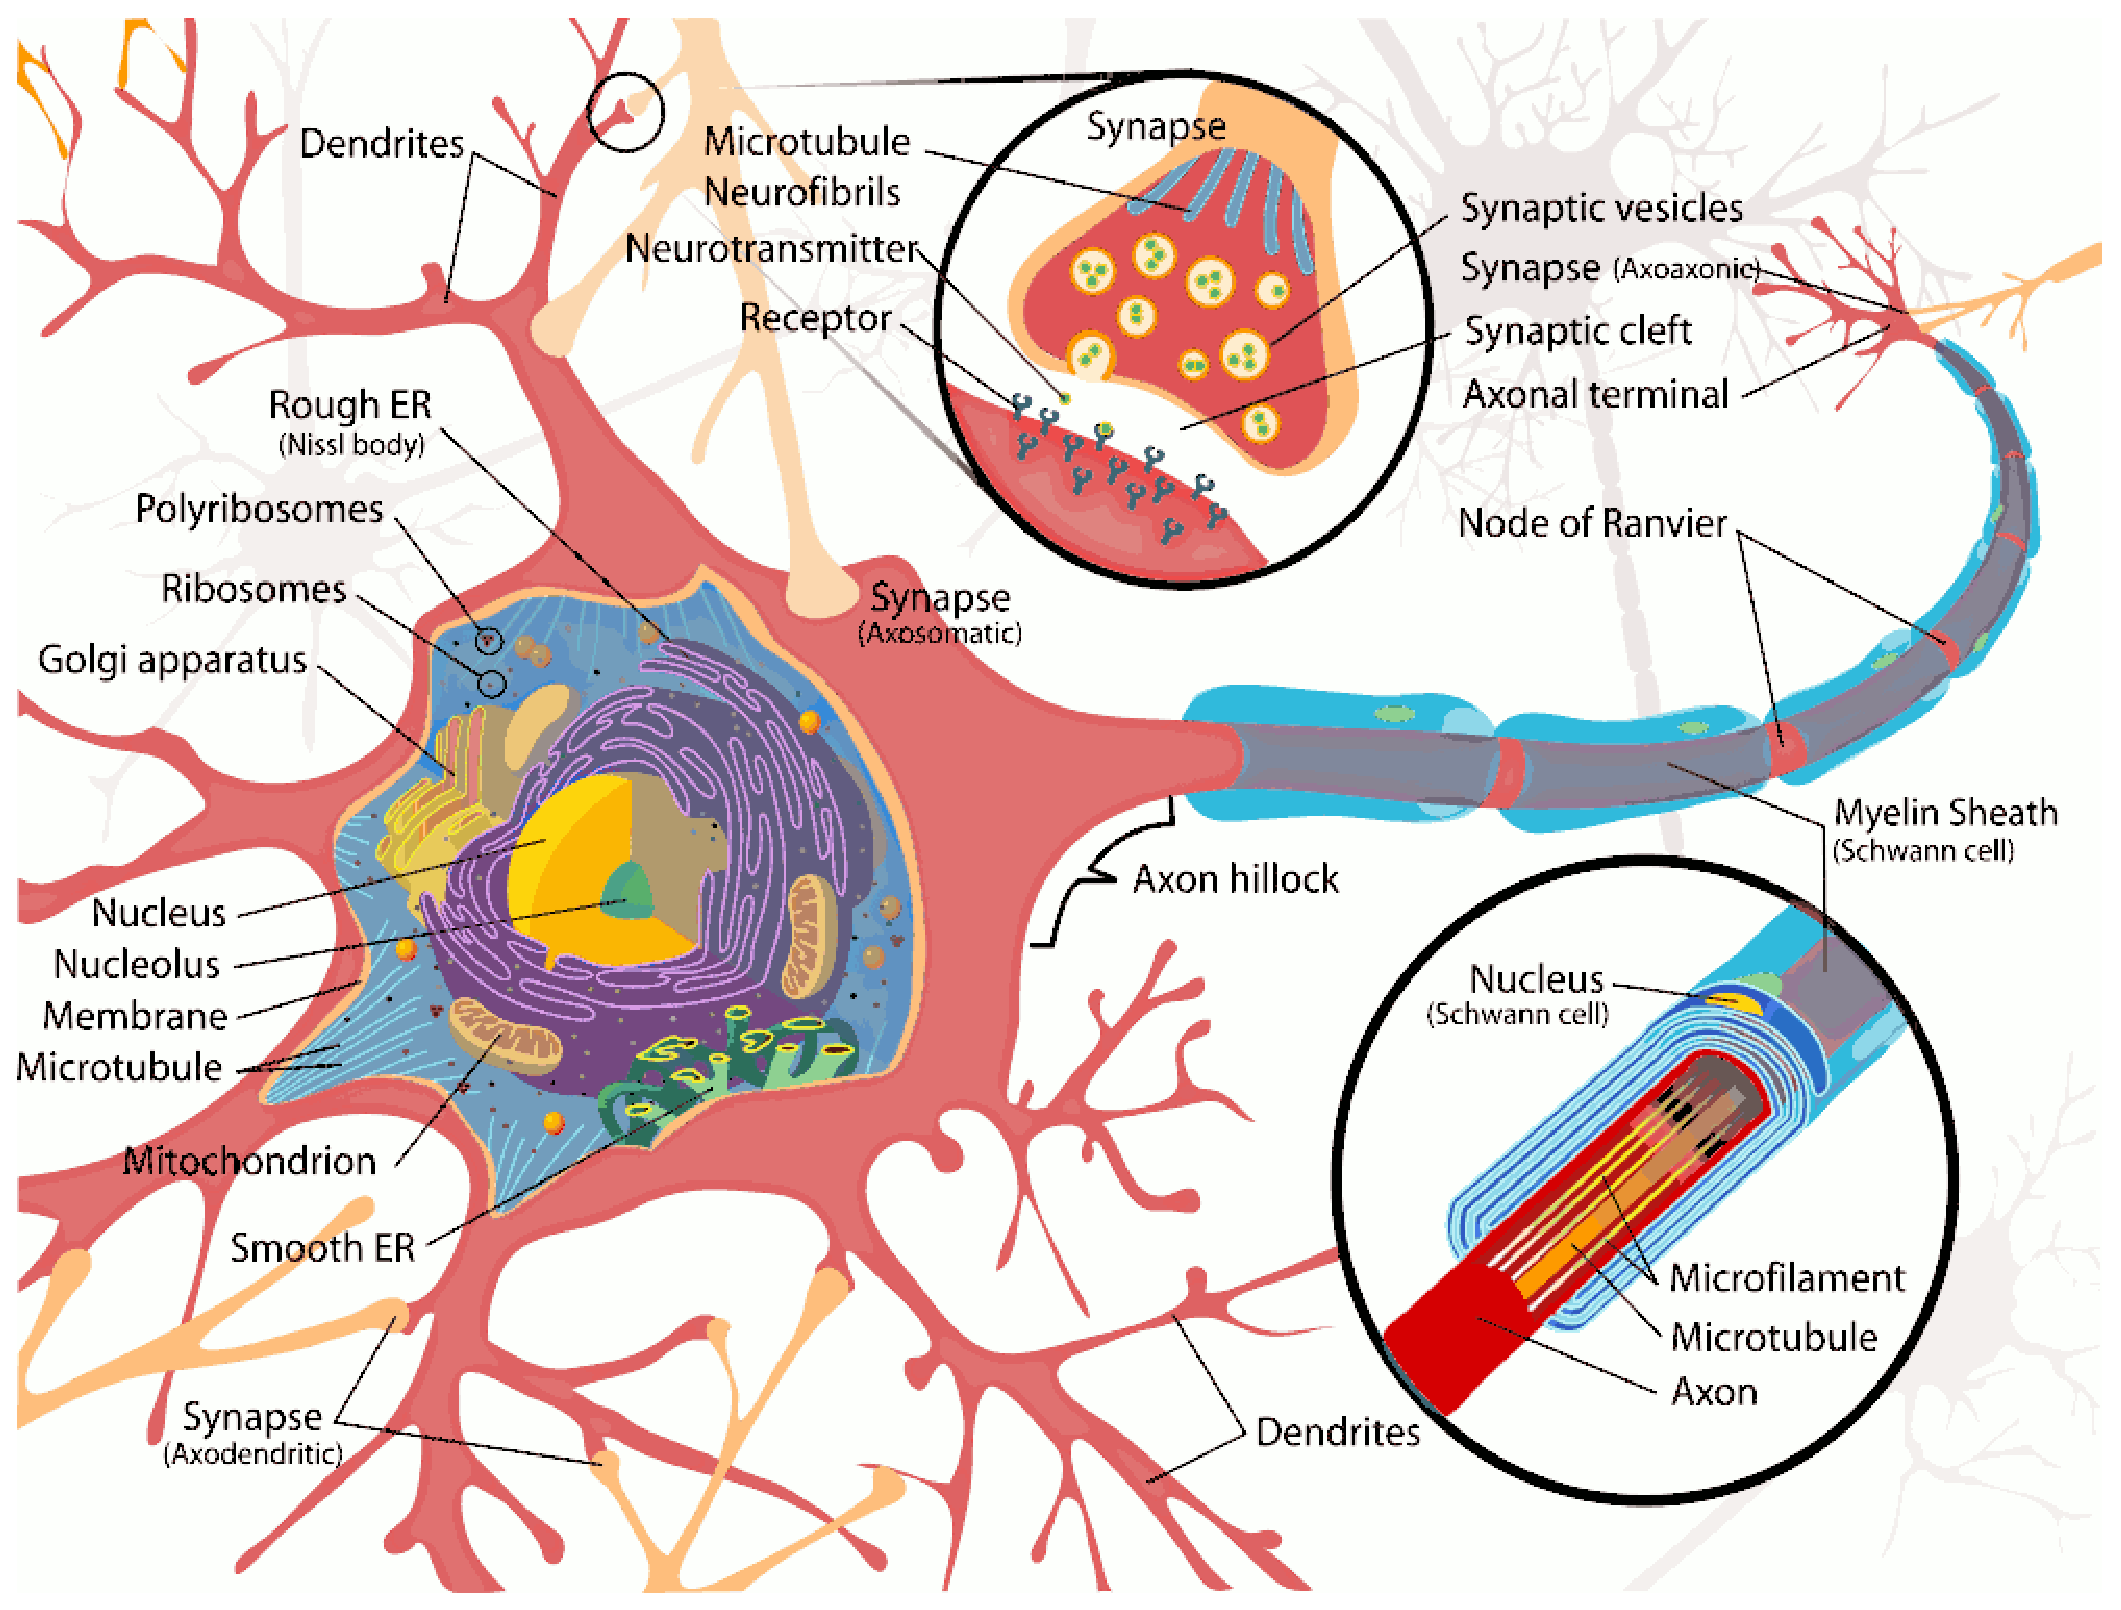
\includegraphics[width=12cm]{Neuron_cell.eps}
  \caption{Diagram of a neuron~\cite{wclipart}}
\end{figure}

\begin{enumerate}
\item Information that is {perceptible to our senses} reaches us; it can be visual (seeing), auditory (hearing), haptic (feeling), olfactory (smelling) or gustatory (tasting).
  The incoming {information density} is dependent on the type of excitation. Olfactory impulses can have about 20 bit/sec, visual input about 10 million bit/sec.
\item The sensory input reaches a \emph{sensory cell}\index{cell!sensory}, which transmits it to a {nerve cell}\index{cell!nerve} and their nerve endings (synapse) in the form of an electrical excitation impulse (spike) (\textbf{Ultra Short Term Memory}).
\item The impulse {circles} between the synapses of different neurons in a {repeating pattern} (\textbf{Short Term Memory}). The nerve impulses circles along fixed paths in the network of the neurons and it leaves {characteristic molecular traces}, which imprint into the brain.
\item These loose, not yet linked connections between the neurons solidify into {stable connections}, the {fissures}. They make up our  \textbf{Long Term Memory}.
\end{enumerate}

\begin{table}[htb]
  \centering
  \begin{tabular}{ll}
    Light & A flame of a candle in about 30 miles (50 km) distance in a dark, \\
    & clear night \\
    Sound & The ticking of a watch, without surrounding noise in about 20 ft \\
    & (6 m) distance \\
    Taste & A tablespoon of sugar in about 2 gallons (7.6 L) of water \\
    Smell & A drop of perfume distributed in a 3 bedroom house \\
    Touch & The wing of a bee which falls from a bit less than half an inch (1 \\
    & cm) on your cheek
  \end{tabular}
  \caption{Approximate recognition threshold of familiar events}
\end{table}

\begin{figure}[htb]
  \centering
  \includegraphics[width=10cm]{Sensoryinformation.eps}
  \caption{Types of sensory information processed by the brain}
\end{figure}
\newpage
\section{Fissures: Visible Burrows in the Cortex of the Brain}

	All learning processes need {time}. During this time the excitation impulse cycles between the neurons gets chemically fixated on the cortex.
	That leads to the conclusion that {repetition} of the material, as homework and so on, is useful, even necessary. 
	This context sheds a new light on {thinking}: {linking information} to higher, more sophisticated information.
	Learning succeeds best in a stress free, {relaxed atmosphere}, which doesn't exclude healthy performance pressure.

        \begin{figure}[htb]
          \centering
          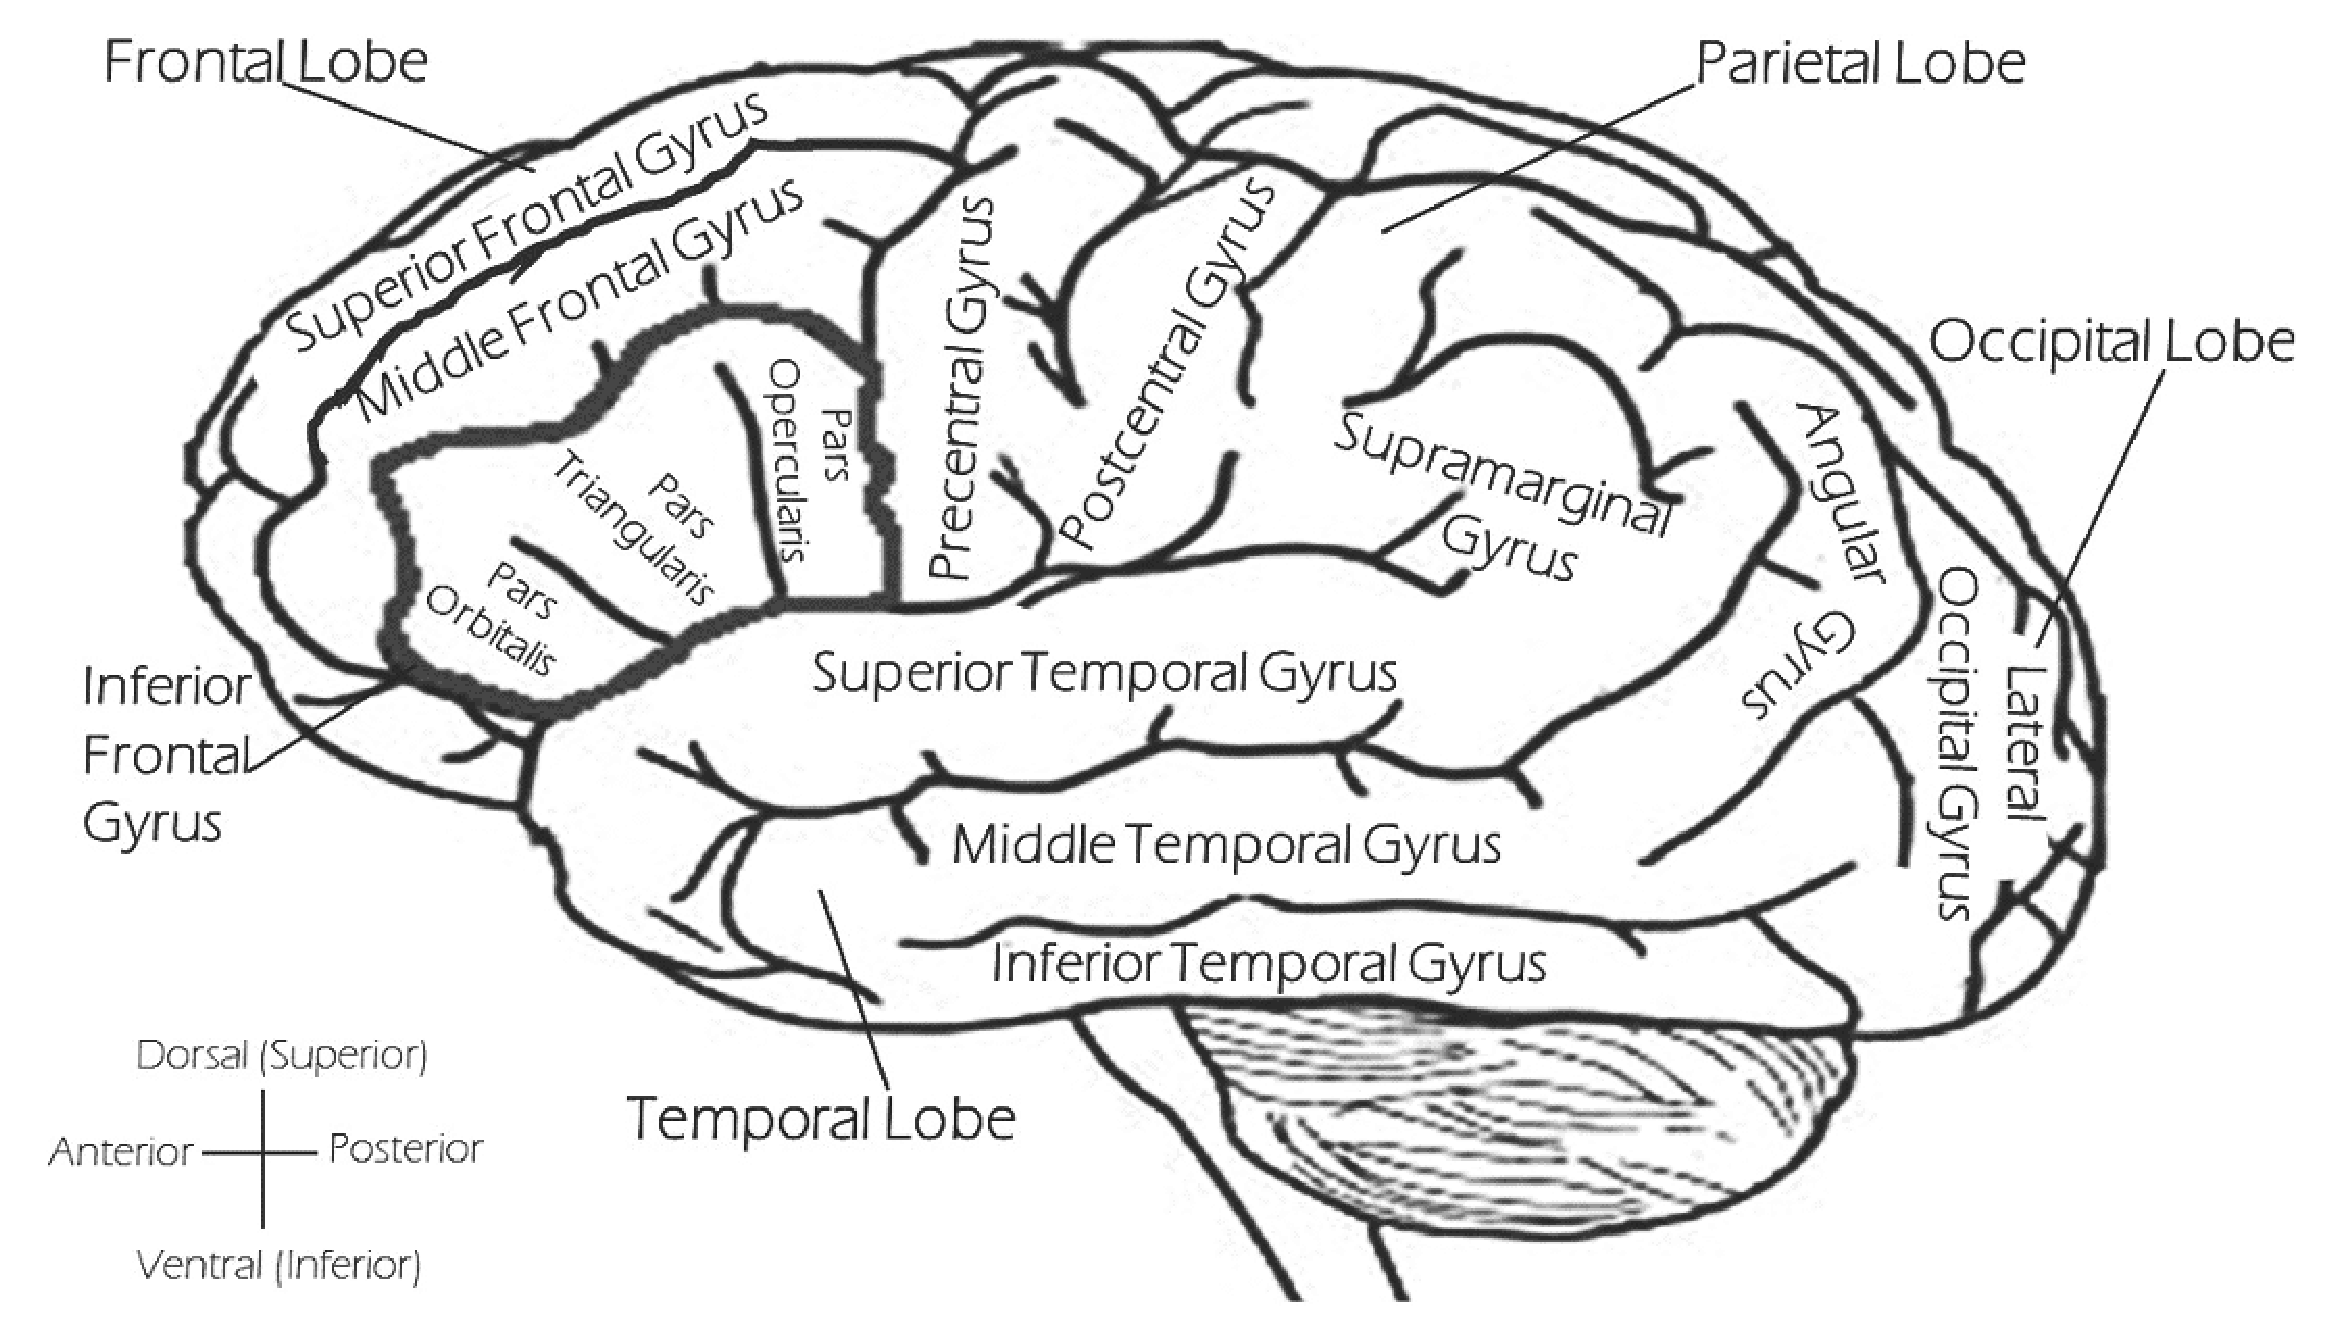
\includegraphics[width=10cm]{brain_labeled.eps}
          \caption{The human brain, labeled~\cite{wclipart}}
        \end{figure}

        The human brain is the most complicated structure know, in average about 44 oz (1245 g) for a female, respectively 48.5 oz (1375 g) for a male brain.\index{brain!weight}
        From a neuro--physiological view all learning and behaviors, all physical processes happen in the brain and get directed by the nervous system.
        The human brain is about triple the weight of the brain of a chimpanzee or gorilla. The Neanderthal had about a more massive brain than modern humans of about 53 oz (1500 g).
        Since the upper paleolithic about 20,000 years ago, there has been a reduction of about 5.3 oz (150 g).
        Out of that reason some scientist assume a permanent reduction of brain mass.\footnote{translated from \textit{Die Evolution des Menschen, Spektrum der Wissenschaft 2003}}

        \setlength\epigraphwidth{.8\textwidth}
        
        \epigraph{Uneducated people are unfortunate in that they do not grasp complex issues, educated people, on the other hand, often do not understand simplicity, which is a far greater misfortune}{\textit{Franz Grillparzer}}
        \setlength\epigraphwidth{.4\textwidth}

        \chapter{The Limbic System}

        The limbic system \index{limbic system} is a collection of complicated structures in the center of the brain, which surround the brain stem like a border (Latin: limbus).
        The limbic system is the \emph{control center of the endocrine\footnote{endocrine: related to the inner secretion of glands}, vegetative\footnote{vegetative: Not subject to conscious control}and mental regulation systems.}
        It processes stimuli from the interior (endogenous) and the exterior of the body (exogenous).
        The limbic system controls the emotional behavior and is the center of feelings.
        
        %Blausen.com staff (2014). "Medical gallery of Blausen Medical 2014". WikiJournal of Medicine 1 (2). DOI:10.15347/wjm/2014.010. ISSN 2002-4436.

        \begin{figure}[htp]
        \centering
         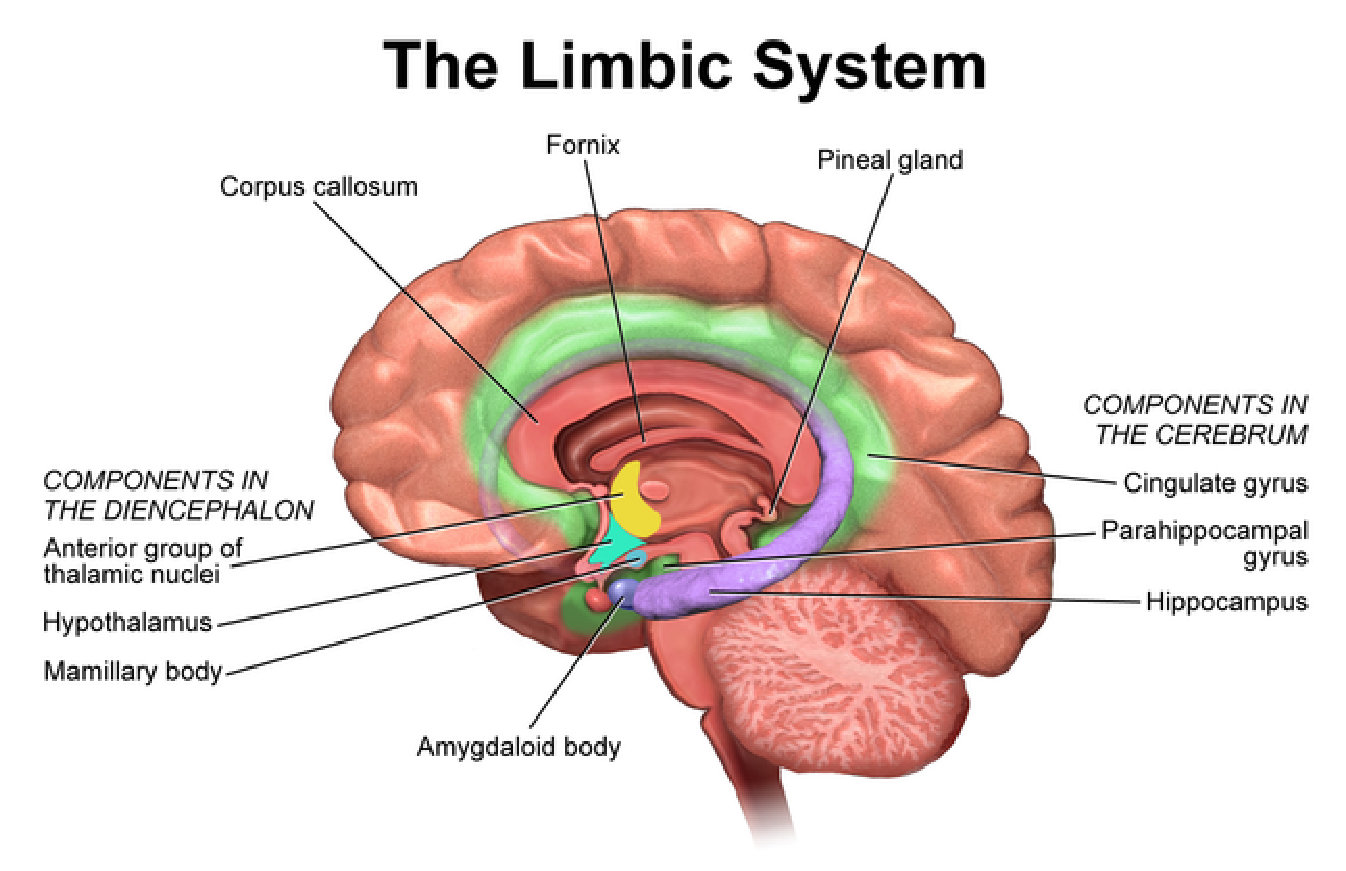
\includegraphics[width=12cm]{LimbicSystem.eps}
          \caption{Diagram of the limbic system~\cite{BlausenLimbic}}
        \end{figure}

        Stress starts already at the sensory organs. An impulse is perceived and it causes in the nerve cells electric signals. They are getting rerouted by the limbic system to the brain for processing.
        The instinctive (vegetative) behaviors in stress situation like fight or flight is also triggered in the limbic system.

        \newpage
        The limbic system\footnote{The limbic system is evolutionary more ancient than the more recent structures of the cerebrum. That's why it's sometimes called the ``reptile brain''.} is in contact to other parts of the brain and regulates through them
        \begin{itemize}
        \item Sleep/awake state
        \item Nutrition
        \item Procreation/Sexuality
          \item Feelings and emotions          
        \end{itemize}

        Disturbances of the limbic system often lead to disturbances of the emotional behaviors. Psychoses and Epilepsy often correlates with disturbance of the limbic system, which can cause  remarkable changes in behavior, like anger attacks, anxiety attacks, hallucinations.

        \newpage
        \mytextbox[0]{Translated from \cite{SpitzerLernen}

          \vspace{5mm}
        The patient H. M. achieved worldwide fame in the neuroscience community. Due to incurable epilepsy the hippocampus and adjacent parts of the brain got surgically removed. On the first glimpse, the patient was totally normal after the operation.
        It turned out, that he was unable to learn any new event.
        The doctors and psychologists visiting him had to introduce themselves every time again; he forgot with whom he dealt during the last visit.
        H. M. could read every day the same journal and was surprised by the novelty of the news.
        Things became very bad, when he moved into a new place. He couldn't locate anything anymore in his new apartment.}

        \vspace{1cm}

        \mytextbox[0]{Translated from the same text \cite{SpitzerLernen}:

          \vspace{5mm}
\noindent        The case Phineas Gage

\vspace{3mm}
        Phineas Gage was a 25 year old lovable and conscientious man --- up to September 13, 1848 where he lost part of frontal lobe in an accident during blast operations.
        He survived the accident, but due to a premature detonation an iron pole destroyed the frontal part of the left brain, entering through his left cheek and exiting at the center of the hairline.

        The day after the accident the pole got found next to the place of the accident, smeared with blood and fatty brain substance. It was about 3 ft (1 m) long and an inch (3 cm) in diameter.

        Phineas Gage survived the accident and was brought to the next village on a ox cart, where he got got emergency care. He was responsive (conscious) pretty much the whole time and ascended the stairs to his hotel room by himself, supported by his house doctor, Dr Harlow.
        Only the big loss of blood lead eventually lead to a strong weariness, but nevertheless he continued talking to his medical doctor:

        ``He endured the agony with inner strength and directed my attention on the whole in his cheek `The iron entered here and went through my head.' His pulse was at this time 60, soft and regular. He recognized me right away and said that he hopes to not be too much hurt.''

        Everybody counted on his quick death and the reports of the progressions in the days and weeks after are more suspenseful to read than any crime fiction. Gage's health decreased; the wound infected; he developed a delirium; the wound got again inspected from top to bottom with a metal probe; the left eye totally went bling, where beforehand it was still able to distinguish light and dark (the iron bar passed behind the eye). The face infected and swell up. Parts of the wound got opened with scissors and stinking puss poured out of it.

        Gage survived. He started eating and drinking (milk and brandy), and was sitting up on the edge of the bed the first time four weeks after his accident and asked for his pants. In November he took the coach to his 30 miles (50 km) remote home town, regardless of having the flu. April of the following year he was visiting his doctor again, which diagnosed apart from the blindness of his left eye, a partial paralysis of the left side of his face and the to be expected scars no further physical symptoms.

        Nevertheless his life completely changed due to the accident, if not to say ruined. He became a totally different human. His personality changes drastically after the accident. He used to be was modest, lovable, reliable and honest, he became after the accident irritable, unreliable, having poor physical and mental posture and unoriented. He stayed afloat up to his death as stable and land worker.

        ``His employers who used to find him the most capable and efficient man remarked his mental changes so strongly that they wouldn't employ him anymore. The equilibrium or the balance between his intellectual capacities and his animal urges seemed to be destroyed. Before his accident he possessed an balanced mind, even if not educated by schools, others saw him as a canny businessman, very energetic and very determined in the realization of all his plans. In this respect, his mind changed so radically and in such an obvious way that his friends said he was `not Gage anymore'.''
      }

      \chapter{The Memory}
      
      \begin{table}[htb]
        \centering
        \begin{tabular}{ll}
          Ultra short--term memory & reacts instantaneously \\
                                   & filters \\
                                   & automated \\
                                   & records 10 to 20 seconds \\
          Short--term memory       & working horse \\
                                   & units of recording 7$\pm$2 seconds \\
                                   & duration of the present: 2 to 10 minutes \\
          Long--term memory & retrieves data \\
                                   & associates known data \\
          & records lifelong \\
        \end{tabular}
        \caption{The different types of memory and their response times}\index{memory}
      \end{table}

      \chapter{Learning and It's Effects}

      \section{What Does the Term `Training' Mean?}

      The term training\index{training} (practice) generally means a measure, which aims at improving the physical, psychological, mental and/or motor capacity.
      In sports it means a regular/repeating physical strengthening with the goal to enhance the physical fitness and the skill levels in the specific sport.

      In the domain of medicine and psychology, there are little distinct terms. Professionals maybe talk of treatment programs, which in my opinion doesn't have too much to do with training.
      Nevertheless we can say, that there are many possibilities to optimize our body in the psychological domain and therefore in the medical domain, too --- through training, for instance Autogenic Training, focused muscle relaxation, posture improvement by practicing gymnastics or yoga and muscle formation by training weights.


      Each form of {learning changes} us. Learning is about  acquiring knowledge and skills and  changing thinking patterns, world views and behaviors. For instance learning French will over time lead to adapting the French way of thinking (the way that French people think).
    
      When I learned something, I have now a skill I didn't have before. I'm able to demonstrate this new skill in with my behaviors.
      Learning also means changing my behaviors and my views respective a person or an object.

      {Inhibitions might hinder a person to produce this new skill or view. This leads to the dilemma: Being able to do versus really doing it. To conclude: {learning always happens in interaction with the surrounding.}}

      Learning doesn't only mean acquiring positive behaviors, meaning behaviors which get interpreted positively by the current surrounding, but as well acquiring negative behaviors.
      This lead to the questions, if me as the teacher can even evaluate, how my teaching activities will influence my students? This is not really possible to know ahead of time.
Due to this reason, I have to foster the student in his/her own context. I promote the sides in him, which already are positive.
      
Learning doesn't always happen in a planned and focused way, often it happens more or less {randomly or under pressure} --- maybe through random encounters and activities, through situations which put up pressure (I have to earn money) or through suggestion.
\emph{Learning is the integration of problems into process} ---  \emph{A problem becomes a task through a learning process}. The problem gets recognized and analyzed and therefore resolvable. The same type of situations will not be seen as problematic anymore after the process of learning: ``No Problems''. Therefore we are again at a form of stress regulation (more in the section~\ref{Le:problem} on page ~\pageref{Le:problem}: ``The definition of the problem'').

\mytextbox[0]{Translated from \cite{SpitzerLernen}
  \vspace{5mm}
  
  \noindent Two groups of two subjects heard one of the following stories, which differentiate in their emotional content.
  
  Story 1: A boy drives with his mum through the city to visit dad who works in a hospital. Once there, he gets demonstrated a series of medical procedures.

  Story 2: A boy drives with his mum through the city and gets hurt very badly in a car accident. They quickly bring him to a hospital, where a series of medical procedures get executed. 

  Both groups had a presentation of a list of medical procedures of the clinic and then got send home. A week later, they were summoned to the lab again and were being asked about the medical procedures of the clinic.

  Even though both stories had the same length and started and ended the same way, the study of the retention rate a week later showed that the people who have heard the emotional story number two were way better at retaining the details of the medical procedures.
}

In this context, let's look at a few theories from psychology, which explain human learning as an acquiring of knowledge or behaviors: the learning theories.
\emph{Pawlow}\index{Pawlow} published the \emph{theory of classical conditioning}\index{classical conditioning} or \emph{signal learning}.
Who hasn't heard of the famous experiment, where Pawlow rang a bell while feeding his dog. Later on, these ``conditional reflexes'' (due to experiences) got triggered by only hearing the signal.


\mytextbox[0]{Translated from \cite{ZimbardoPsych}
  \vspace{5mm}
  
  \noindent The Russian physiologist Ivan Pavlov (1849--1936) actually didn't intend to research neither classical conditioning nor another psychological phenomena. He discovered classical conditioning while doing research on digestion, for which he got the Nobel price in 1904.
  
  Pavlov developed a method, which allowed to examine digestion conditions on dogs. He implanted tubes into their glands and digestive organs to extract the body fluids out of the body and therefore make it possible to measure and analyze these samples. In order to produce these secretes, Pavlov applied meat powder to the mouth of the dogs.

  After applying these treatments several times, Pavlov started to discover an unexpected behavior of his dogs. They started to produce saliva even before they were given the meat powder. In fact, they started to produce saliva only seeing the food, later upon seeing the assistant who brought the food, and even just the sounds of the assistant's steps.
  Each stimulus, which precedes on a regular level the food, could increase the flow of saliva. Pavlov discovered so to say by chance, the learning can be caused by the association of two stimuli.

  Pavlov had the capacity and the thirst for knowledge to research this phenomena. He ignored the advice of the leading physiologist of his time, Sir Charles Sherrington, to abandon the useless research of ``mental'' secretions.
  Pavlov quit his work on digestion and by doing so changed the face of psychology forever.
  
}

\emph{Skinner}\index{Skinner} phrased the theory of \emph{learning through success}\index{learning!through success}. It says, that if a behavior is rewarded, it will more likely be repeated that if it gets punished.

\mytextbox[0]{Translated from \cite{ZimbardoPsych}
  \vspace{5mm}
  
  \noindent
  While being associated with reinforcement or punishment certain stimuli which precede a specific reaction gain the ability to determine the context of the behavior. These stimuli are called discriminatory clue stimuli.

  Organisms learn that their behavior and the absence of other behavior very likely has a certain effect on the surroundings. For instance in the presence of a green signal the behavior of crossing the intersection gets reinforced. Is the signal red, this behavior gets punished --- it can end in a fine or an accident. Skinner named in 1953 the effects of discriminatory stimulus, behavior and consequence as triple contingency and believed, that those can explain most human behaviors.
  }

  In the view of \emph{Bandura}\index{Bandura} we learn by \emph{observing}. We observe other people at a certain behavior and whether it gets rewarded or punished we apply this behavior ourselves or not. This ``learning by model''\index{learning!by model} requires that we are capable and ready to execute the observed behavior.

\mytextbox[0]{Translated from \cite{ZimbardoPsych}
  \vspace{5mm}
  
  \noindent A classic demonstration of human learning by observation happened 1963 in the lab of Albert Bandura. After kids could observe adults pushing, beating and stomping on a plastic clown puppet called Bobo, they showed higher number of similar incidences themselves than kids of a control group who didn't see the aggressive models.

  There's no questions, that we learn a lot --- prosocial (helpful) as well as antisocial (hurtful) behaviors --- by model; but there are many models in the world. Which variables determine, which models most likely will influence you?
  Research delivers the following general consequences:

  The behavior of a model will be especially influential, when
  \begin{itemize}
  \item there's a perception that the behavior brings reinforcing consequences;
  \item the model gets perceived as positive, popular and respected;
  \item there's a perception that there are similarities with respect to attributes and traits of the model with the observer;
  \item the observer gets rewarded for putting his attention to the behavior of the model;
  \item the behavior of the model is well visible and salient --- when it contrasts as a clear image against the background of competition between models;
    \item it is possible for the observer to imitate the behavior.
  \end{itemize}
  
}

  
\chapter{The Definition of the Problem}\label{Le:problem}

A \emph{problem}\index{problem}\footnote{Greek = what's presented, brought in front of you} gets created, when the knowledge or the skills is missing to achieve a specific goal.
It shows how important it is in our lives to train \emph{creativity}, in order to find the way to \emph{several possible solutions}.

\epigraph{Learning is like rowing against the current. As soon as you stop, you drift back.}{\textit{Benjamin Britten}}

The problem is characterized by the tension between the goal and the stating situation, which is different from the goal.
The process of eliminating a problem by overcoming the described tension is called \emph{solving a problem}.\index{problem!solving}
It is evident, that in this tension there's a certain pressure (stress) created, which gets called the inhibition to solve the problem.

\epigraph{The problem is serious, the solution cheerful.}{\textit{Bert Hellinger}}

A problem is not the same as a task. We have rules for a task, to come to the solution.
In order to recognize the rules, it's important to relieve the pressure (stress) as soon as possible. Otherwise an overburdening of the pressure doesn't allow for a solution anymore.
As we all have a different amount of knowledge, problems as well as tasks are \emph{specific to the person}. This proves that something that can be a huge stress can be solved elegantly by another person.
We distinguished between problems which concern only one individual from the ones which are a problem for many people.

Changing the inner views through targeted and skilled transforming \emph{problem based thinking} to \emph{task based thinking} and eventually to \emph{solutions based thinking} can be assisted by training metacognitive elements (see section~\ref{metacognitive} on page~\pageref{metacognitive}).

If you can split up a problem in multiple parts, it's called a \emph{hierarchical problem}. if this isn't possible, then it's a \emph{elementary problem}.

        \setlength\epigraphwidth{.8\textwidth}
        \epigraph{The vengeance
          
          \vspace {5mm} \noindent A small trader writes a letter to a big supplier:
          
  Dear Sir,

  Four weeks ago I ordered a box of curd soap. It still didn't arrive. My stock is depleted and I have significant losses through your negligence. We, the small ones, have to be contend to be treated like dirt by the big traders.
  
  The letter went on for several pages like this. After the signature, there was a little note:
  
  P.S. In the meanwhile I found the delivered box with the soap.}{\textit{Bert Hellinger}}
        \setlength\epigraphwidth{.4\textwidth}

        \chapter{Training and practicing}

        From the mentioned theories of learning and the definition of the problem, we see that training (practicing)\index{training}\index{practicing} is central to achieve certain given or self defined goals.


        Based on the example of training of social skills we can get leads to where the inhibitions, disturbing factors or promoters are to be found in us.

        There are many difficulties arising for people with a psychotic or neurotic disorders or just people with daily problems just from the fact, that they are inhibited, maladjusted or insecure in their \emph{social behavior}.

\mytextbox[0]{Translated from \cite{Rueckle}
  \vspace{5mm}
  
  \noindent Social skills are reactions or patterns of reactions which allow it a person to succeed while approaching others or in the interaction with others. Covered by it is what to say or to do in a given situation (content), how (style) and when (timing) it is to be said or done. And how to assure that in the conversation partner the desired reactions gets triggered (consequences).
}

\epigraph{Our wishes are the premonitions of the capacities, which are inside of us.}{\textit{Johann Wolfgang von Goethe}}

One of the most prevalent problems with social skills is lacking confidence and the inability to put the thoughts and wishes into words in a clear, direct and not aggressive manner. Even though problems that adults have in that domain often got caused in the childhood, it's nevertheless important to diligently work on them.

\textbf{People with insufficient social skills, which is an important, often unconscious stressor, can be lead with training to a more successful behavior.}

\vspace{1cm}

\mytextbox[0]{Translated from Bert Hellinger
  \vspace{5mm}
   
  \noindent Bedazzlement

  A circus acquired a polar bear. Given that they needed him only for exhibitions, they put him in a cage.
  It was so narrow that he couldn't even turn around in there. So he continued to go two steps forward in his cage, then two steps backward.

  
  After many years they had pity with the polar bear and sold him to a zoo. There he had a big cage and a big compound. But he continued to go two steps forward, then two steps backward. Another polar bear asked him: ``Why are you doing this?'' he answered: ``That's because I was trapped for so long in a little cage.''
  }

\subfile{Metacognitive.tex}

\chapter{The Signification of the Colors}

If you imagine a landscape in blue, it has a different effect on you, than if you imagine a landscape in red. Colors\index{color} carry a statement, even if they don't get felt by all people in the same way and intensity. So, colors can \emph{transmit} a quality, but they can \emph{support} us with their quality.

A possible categorization for the colors:

\begin{description}
\item[Red:] The color of the vital will to action, of love,  emotionality, assertiveness, excitation and passion.
\item[Orange:] The color of self--confidence and of creativity, of warmth and ambition, of power and zest for action.
\item[Yellow:] The color of thinking, sensitivity, of the mind, being full of ideas and ideals, changes, the wish of liberation, hope and expecting happiness.
\item[Green:] The color of introspection, of freedom. It contains peacefulness, adaptability, being in equilibrium, serenity, sensitivity, open--mindedness and happy detachment.
\item[Blue:] Shows, calmth, peace, the need to recover, openness, silence, fidelity, depth, selflessness and capacity to surrender.
\item[Indigo:] Indigo is the color of the belief, the capacity to immerse, security, of the silent existence. Social thinking and actions are associated with this color. it contains also humanity, altruism, charity, sincerity, honesty, and justice. 
  \item[Violet:] Religious feelings, serve, self--sacrifice, abstinence and asceticism lie in this highest color. Mystics, insight, perfection and salvation are attributed to this color.
  \end{description}

  This choice of colors wasn't done in an arbitrary way. They are the colors of the rainbow. Many people are persuaded, the part of the human body are the subtle energy center (``chakras''), which are often represented as rotating vortexes. Each of these energy center has a color associated and a gland of the human body, depending on it's location.

 \begin{table}[htb]
  \centering
  \begin{tabular}{llll}
    Root--chakra & between genitals and anus & adrenals & red \\
    Sacral--chakra & below the navel & gonads & orange \\
    Solar plexus--chakra & above the navel & pancreas & yellow \\
    Heart--chakra & middle of the chest & thymus gland & green, pink \\
    Throat--chakra & on the throat & thyroid gland & light blue \\
    Third eye--chakra & between the eye brows & pituitary gland & indigo blue \\
    Crown--chakra & top part of the head & pineal gland & violet, white
  \end{tabular}
  \caption{The chakras of the human body.}
\end{table}


\epigraph{I don't mind almost believing that you can feel colors; their unique quality would only be confirmed even more. You can also taste them. Blue becomes alkaline, a yellow--red would taste sour. All manifestations of the essentiality are related.}{\textit{Johann Wolfgang von Goethe}}

\chapter{The Hemispheres of the brain}

The human cerebrum is split in half, the \emph{hemispheres}\index{brain!hemispheres}. Each half has four lobes: The \emph{frontal, parietal, temporal and the occipital lobe}. They are separated by the longitudinal fissure.A white substance which consists of motor and sensory axons which serve as connectors {corpus callosum} connects the two. The cerebrum works in a \emph{cross--over pattern}. Half of the body is controlled by the opposite hemisphere. Research showed, that each hemispheres process information in a unique way.

\begin{figure}[htb]
  \centering
  \includegraphics[width=5cm]{brain_hemispheres.eps}
  \caption{The hemispheres of the brain and the longitunal fissure\cite{needpix}.}
\end{figure}


The ``logical hemisphere'' (typically left) organizes language, reading, writing, calculations, musical capacities and analytical thinking.

The ``Gestalt--hemisphere'' (typically the right one) is associated with feelings, connections, language, spatial perception, intuition, thinking in pictures and synthesis.


\end{document} 